\documentclass[../thesis.tex]{subfiles}
\begin{document}
\chapter{Overview of Organic Semiconductors}\label{sec:orgSemi}

\section{Organic Semiconductors}

Organic molecules are broadly classified as molecules primarily composed of carbon.\supercite{Pope1999}.
These molecules can range dramatically in size, and are often split into small molecule ($m_w<1$ kg/mol) and polymers.
For organic electronics, both categories can be used, but this thesis will focus on small molecules, as that is the primary interest of commercial devices.

\begin{wrapfigure}{r}{.5\textwidth}
\centering
\includegraphics[width=.48\textwidth]{orgSemiconductors/benzene}
\caption{Molecular orbitals of benzene.  The left figure shows the 6 out of plain p$_z$ orbitals, and the right image shows the delocalized $\pi$-bond.\supercite{benzene}}
\label{fig:orgSemi_benzene}
\end{wrapfigure}

To exhibit semiconducting behavior, electrons must be delocalized within the system.\supercite{Neamen1992}
For organic molecules, this is achieved through overlapping p orbitals from carbon.  
Through alternating single and double bonded carbon, hybridized 2p and 2s orbitals form three sp$^2$ orbitals and leave one unhybridized p$_z$ orbital.
The remaining p$_z$ orbitals can interact, forming a $\pi$-bond and delocalizing of the electron cloud, known as \textit{conjugation}.
An example of this is shown for benzene, in Figure \ref{fig:orgSemi_benzene}.

When this conjugation and blending of molecular orbitals occurs, discrete energetic states mix, resulting in multiple energetic states.\supercite{Kittel2005,Wallis2000}
The formed energetic states can be grouped into bands of allowed energies.
%With more delocalization comes more states resulting in bands of allowed electron energies.
In order to exhibit semiconducting behavior, the resulting bands should have a set of states filled with electrons separated by a gap from a band of unoccupied states.
For the organic small molecules of interest to this study, delocalization occurs on individual molecules, resulting in less delocalization and thus much narrower bands than would be observed in a typical semiconductor, such as silicon or germanium, but the concept remains the same.
In organic molecular semiconductors, the highest occupied molecular orbital (HOMO) and lowest unoccupied molecular orbital (LUMO) are analogous to the valence and conduction bands of inorganic semiconductors in terms of their roles for electrons and holes, though their operation is vastly different.
The HOMO is filled with electrons and the LUMO is empty in the ground state.
When excited, electrons can be transported through the LUMO levels.
This will result in an electron vacancy in the HOMO, known as a \textit{hole}

Films are held together by intermolecular dipole-dipole interactions, known as van der Waals forces.
These forces can involve both permanent and induced dipoles.
This weak binding with the molecules displaying semiconductor properties as individual molecules allow these films to be flexible.
Traditional crystalline semiconductors rely on the periodicity of the lattice to exhibit energy bands.  
This is a huge advantage of organic semiconductor devices, allowing for a variety of unique applications.

\section{Charge Transport}

Charge transport in organic semiconductors can take on a variety of behaviors, depending on material and morphology.\supercite{Pope1999,Mark1962}
Two regimes of operation are typically expected, being band transport and hopping transport.  
As disorder increases, a shift from band to hopping transport is expected.

\subsection{Band Transport}

Band transport is expected in most atomic crystals, and is thus extensively characterized for inorganic semiconductors.\supercite{Kasap1997}
In a crystal, a periodic energy structure is maintained throughout the entire structure.
This creates a delocalization of the electron wavefunction across the crystal and electrons have a mean free path that extends for multiple molecular spacings.
Because of this freedom of charge movement, charges can be directly accelerated through the crystal by an electric field, $\vec{E}$.
This creates a current density of 

\begin{equation}
\vec{J}=qn\mu \vec{E},
\end{equation}

where $q$ is the unit charge, $n$ is the charge carrier density, and $\mu$ is the charge mobility.
Typically in these materials, the mobility decreases with temperature as vibrations in the crystal lead to more scattering of the electrons.


\subsection{Hopping Transport}

In less ordered materials, there is substantially less symmetry and periodic potentials and electron distributions are much more confined .
In this case, each molecule serves as an individual energetic well, and for transport, charges are forced to conduct individual hops to neighboring molecules. 
This dramatically reduces the mobility compared to band transport.
With temperature, mobility follows an Arrhenius dependence that can be split into a field dependent and field independent term as

\begin{equation}
\mu \propto \exp\left(-\frac{E_a}{k_BT}\right)\exp\left(\frac{\beta\sqrt{E}}{k_B T}\right)
\end{equation}

with $E_a$ being the hopping activation energy and $k_B$ being the Boltsmann constant.
$\beta$ is a constant and $E$ is the electric field.

These two transport mechanisms account for very different physics.
Organic semiconductors can operate in either regime.
Temperature dependent current measurements can be conducted to illuminate mechanism, and often morphology can be a good predictor.
In amorphous organics, a hopping mechanism can typically be assumed.

\section{Excitons}\label{sec:excitons}

\begin{wrapfigure}{r}{.3\textwidth}
\centering
\includegraphics[width=.3\textwidth]{orgSemiconductors/exciton}
\caption{Schematic view of an exciton.  $S_0$ and $S_1$ are the ground and first singlet excited state, respectively.}
\label{fig:orgSemi_exciton}
\end{wrapfigure}

In organic semiconductors, a critical component of light formation or absorption is the formation of a bound excited state, called an \textit{exciton}, shown schematically in Figure \ref{fig:orgSemi_exciton}.
An exciton consists of a hole in the HOMO bound to an electron in the LUMO.  
Due to the low dielectric constant ($\epsilon_R\approx 3$), excitons in organic materials are highly localized and have large binding energies, >100 meV.\supercite{Turro1991a,Reineke2007,Hains2010,Gregg2003a}
These excitons can be relatively long lived at room temperature, with characteristic lifetimes, $\tau$ ranging from ~0.5 ns - 1 ms. \supercite{Song2011,Park2010,Ryasnyanskiy2011,Wang2013,Erickson2014,Furno2012,Baldo2002,Mikhnenko} 
Because of these long lifetimes, the dynamics of excitons, both in their interaction as well as decay into light or heat, are important to the understand of organic semiconductor behavior.
Excitons that reside on a single molecule are known as ``Frenkel'' excitons, while an exciton spanning neighboring molecules is known as a ``charge-transfer'' exciton.
Excitons spanning larger spatial extents are not seen in amorphous organic semiconductors.

\newpage

\subsection{Singlets and Triplets}
\begin{wrapfigure}{r}{.5\textwidth}
\centering
\includegraphics[width=.48\textwidth]{orgSemiconductors/triplets}
\caption{Spin vectors for the possible spin state combinations of an electron and a hole.  The orientation of the cone represents spin up or down, while the cone indicates the relative phase of the precession in angular momentum.  Triplets all yield a total spin of S=1 while the single has $S=0$.}
\vspace{-40pt}
\label{fig:orgSemi_spin}
\end{wrapfigure}

Electrons and holes have a spin of $S=\pm 1/2$.  
These spins can combine into four possible spin combinations, shown in Figure \ref{fig:orgSemi_spin}
Three of these states have spin $S=1$ and are called \textit{triplets} due to the degeneracy.
The remaining state is called the \textit{singlet}, with $S=0$.
Electrically, excitons are formed from loose electrons and holes, and from simple statistics, form 75\% triplets and 25\% singlets.\supercite{Zhang2014a,Nakanotani2013,Mehes2014}
Optically, due to spin conservation from an $S=0$ photon, only singlet excitons are initially formed.




\vspace{40pt}

\subsection{Electronic Transitions}
\begin{figure}[ht]
\centering
\includegraphics[width=.6\textwidth]{orgSemiconductors/jablonski}
\caption{Jablonski diagram for an organic semiconductor. Fluorescence and Phosphorescence are both depicted, though in some systems, phosphorescence is not observed.}
\label{fig:orgSemi_jablonski}
\end{figure}


Figure \ref{fig:orgSemi_jablonski} shows the energy landscape available to excitons in an organic semiconductor.
The singlet manifold is shown on the left, with the first three electronic energy levels shown as $S_0$, $S_1$,  and $S_2$.
The vibronic levels of these states are labeled as $0,1,2$.
The ground state is depicted as $S_0$.
Absorbed photons create excitons in the $S_1$ and $S_2$ manifolds.
When making electronic transitions, electrons are assumed to start from the lowest vibronic state, by Kasha's rule.

Once created, excitons rapidly convert from higher energy states back to $S_1$, losing addition energy to phonons through internal conversion.
From $S_1$, excitons can decay back to the ground state either by non-radiative or radiative means, known as fluorescence.
The balance of radiative ($k_r$) and non-radiative ($k_{nr}$) rates determines the photoluminescence efficiency by the equation

\begin{equation}
\pl=\frac{k_r}{k_r+k_{nr}}.
\label{orgSemi_pl_efficiency}
\end{equation}


Typically, $k_r$ is on the order of $10^8$ s$^{-1}$ for singlet excitons, resulting in lifetimes on the order of 10 ns.\supercite{Turro1991a,Menke2013}

Since triplet excitons have an electron and a hole that share the same spin state, they are subject to the exchange interaction, increasing the separation and reducing repulsion, resulting in a lower energy state.
In order for a singlet exciton to transition into a triplet, a flip in spin is needed.  
This transition is promoted in systems exhibiting spin-orbit coupling.
Spin-orbit coupling involves coupling of the electron spin with the angular momentum of the orbit, allowing the spin to be reversed.
This is much more common as the atomic number increases, and is commonly seen in heavy metal atoms.
As spin-orbit coupling becomes more prominent, excitons are allowed to freely transition between the singlet and triplet state, and can become mixed.

\begin{wrapfigure}{r}{.35\textwidth}
\centering
\includegraphics[width=.28\textwidth]{orgSemiconductors/ir(ppy)3}
\caption{\irppy, a commonly used OLED molecule with an excited state which exhibits MLCT.}
\label{fig:orgSemi_irppy}
\end{wrapfigure}

In coordinated molecules involving ligands off of a heavy-metal core, it is possible to form Metal-Ligand Charge Transfer states (MLCT).
%This type of charge transfer state is common in molecules  with high energy metallic d-states and low energy $\pi^*$ orbitals.
The high energy d-states of the metal atom promote spin-orbit coupling.
Molecules exhibiting MLCT states have excited states that reside partially on the metal atom, allowing spin flipping to occur, and promoting singlet-triplet mixing.
An archetypical MLCT exhibiting molecule, Tris[2-phenylpyridinato-C$^2$,N]iridium(III) (\irppy) is shown in Figure \ref{fig:orgSemi_irppy}.

The triplet state is considered a ``forbidden state'' for emission, and is quantum mechanically disallowed in first order approximations due to the conservation of spin between the triplet ($S=1$) and the ground state ($S=0$).
However, these spin transitions can occur, especially with significant spin-orbit coupling.
Since an additional spin flip is required, the radiative rate of emission from the triplet state is usually $k_r=10^6$ s$^{-1}$ or longer, dependent on the ability of the molecule to undergo a spin transition.
This slower rate of radiative emission when compared with the singlet state makes phosphorescence much more competitive with non-radiative loss pathways.
Because of this, without molecules that promote spin-orbit coupling, triplet emission is extremely inefficient and is not visible at room temperature.
However, at low temperature (10K)\supercite{Holmes2003,Turro1991a,Goushi2004d,Frankfurt1989,Padhye1956} or with non-radiative pathways reduced,\supercite{Reineke2014} the triplet emission can be observed.
This can be exploited for the measurement of the triplet state energy, as discussed in Appendix \ref{sec:triplets}.


The transition from a triplet back into a singlet is also possible, and is known as \textit{reverse intersystem crossing}.\supercite{Chan2018,Lee2016,Inoue2016,Zhang2014a,Mehes2014,Zhang2012c,Endo2009,Li2013,Nakanotani2013,Nasu2013}
Though this is energetically unfavorable in most molecules, due to the energy difference of the singlet and triplet, an exciting area of emitter research is in Thermally Activated Delayed Fluorescence (TADF).
In TADF molecules, the singlet-triplet energy difference ($\Delta E_{ST}$) is below the thermal energy at room temperature, and allows promotion back into the singlet state.
Efficient transition between the singlet and triplet is observed in TADF systems despite the lack of spin-orbit coupling introduced by MLCT states.  
This is because the mixing coefficient between the singled and triplet can be expressed as\supercite{Uoyama2012}

\begin{equation}
\lambda=\frac{H_{SO}}{\Delta E_{ST}}
\end{equation}

where $H_{SO}$ is the spin-orbit interaction.  
In TADF molecules, since $\Delta E_{ST}$ is small, significant transfer can still be observed.
These materials are advantageous in OLEDs because they allow electrically formed triplets to convert to a singlet for emission without using expensive rare-earth metals.

\subsection{Exciton Transport}

As excitons are charge neutral and not subject to drift in an electric field, their transport relies upon a diffusive process in organic materials.
Diffusion relies on being able to transfer excitons from a \textit{Donor} molecule which has the initial excitation onto an \textit{Acceptor}.
Three mechanisms are common to facilitate this transfer: cascade energy transfer, Dexter transfer and F\"{o}rster transfer.
All three of these mechanisms can contribute to exciton transport, but typically one is dominant for a given material.

\subsubsection{Cascade Energy Transfer}

Cascade energy transfer consists of exciton emission in the form of a photon being reabsorbed by another molecule.\supercite{Turro1991a}
The efficiency of this transfer depends on the photoluminescence efficiency of the donor molecule to form a photon, as well as absorption of the acceptor molecule at the photon energy.
Of the three mechanisms, this is the longest range and can allow transport for 10-100 nm, though relies on propagation of the photon through the surrounding media.

\subsubsection{Dexter Transfer}

Dexter transfer is the shortest range process and describes direct physical transfer of the excited state from the donor to the acceptor.
The rate of Dexter transfer can be written as\supercite{Turro1991a}

\begin{equation}
k_D=Ke^{-2R_{DA}/R_0}\int{ E_D(E)A_A(E)dE}
\label{eqn:dexter_rate}
\end{equation}

where $K$ is dependent on the specific orbital interactions, $R_{DA}$ is the separation of the donor and acceptor, $R_0$ is the characteristic length scale for orbital overlap, normalizing the rate to other energy loss pathways, $E_D$ is the donor emission spectrum, $A_A$ is the acceptor absorption spectrum, and $E$ is the energy.
As can be seen from the exponential dependence, Dexter transfer requires spatial overlap of the electron density of the two molecules, limiting Dexter transfer to nearest neighbors, typically.

Because Dexter transfer involves the direct exchange of charges, the spin state of the electron and hole are preserved.
Additionally, since no intermediate photonic state is required, excitons with $S\neq0$ (triplets) can be transferred.
Dexter transfer is typically the dominant mechanism of transport for triplet excitons.

\subsubsection{F\"{o}rster Transfer}

F\"{o}rster resonance energy transfer (FRET) describes transfer of an exciton via an overlap in the dipole field of the donor with the acceptor molecule.
In this process, the dipole interaction can be thought of as a transmission and receiver antennae.  
The exciton on the donor causes an oscillation in the dipole field which excites an electron in the acceptor to become excited.  
This excitation on the acceptor relaxes the donor to the ground state.

The rate of F\"{o}rster transfer can be expressed as\supercite{Menke2013,Mullenbach2013,Menke2016}

\begin{equation}
k_F(d)=\frac{1}{\tau d^6}\frac{9\eta_{PL}\kappa^2}{128\pi^5n^4}\int{\lambda^4E_D(\lambda)A_A(\lambda)d\lambda}=\frac{1}{\tau}\left(\frac{R_0}{d}\right)^6
\label{eqn:forster_rate}
\end{equation}

where $\tau$ is the exciton lifetime, $d$ is the distance between the donor and acceptor, $\eta_{PL}$ is the photoluminescence efficiency, $\kappa$ is a factor depending on the dipole orientation, $n$ i s the index of refraction, $\lambda$ is the wavelength, $E_D$ is the donor emission,  and $A_A$ is the acceptor absorption.
The integral expression in Equation \ref{eqn:forster_rate} is an expression of Fermi's golden rule and requires that the initial and final spin states be the same.
Therefore, F\"{o}rster transfer is typically restricted to singlet excitons.
Because of this field transfer of singlet excitons, FRET is often described as a transfer of a ``virtual photon''.\supercite{Pope1999,Turro1991a}

F\"{o}rster transfer typically transfers excitons up to 10 nm apart, though is a strong function of distance.\supercite{Menke2013,Luhman2011}
The radius at which the rate of FRET is equal to other loss pathways is called the F\"{o}rster radius ($R_0$).



\subsection{Excitonic Interactions and Quenching Processes}\label{sec:orgElec_quenching}

Excitons are subject to a variety of bimolecular processes and loss pathways.  
This section seeks to outline these processes.

\subsubsection{Exciton-Exciton Annihilation}

\begin{wrapfigure}{r}{.5\textwidth}
\centering
\includegraphics[width=.48\textwidth]{orgSemiconductors/exciton-exciton}
\caption{Exciton-exciton annihilation process.  The energy of two excitons is transferred all onto a single molecule, forming a single exciton.  This exciton then relaxes, emitting heat.}
\label{fig:orgSemi_TT}
\end{wrapfigure}


Exciton-exciton annihilation involves the transfer of energy of one exciton onto an already excited molecule.  
This forms a single exciton with twice the energy, promoting the exciton into the second excited state.
This exciton quickly relaxes back into the first excited state, releasing the excess energy as heat.

Exciton-exciton annihilation is a bimolecular process and has a rate dependent on the exciton density squared of $K=k_{EE}N_{ex}^2$.\supercite{Reineke2007}
In this expression, $k_{EE}$ is the material dependent rate constant.
Exciton-exciton annihilation can affect both singlet and triplet excitons, though is typically more prominent in phosphorescent systems due to the longer exciton lifetime.


\subsubsection{Triplet Fusion and Singlet Fission}
\begin{wrapfigure}{r}{.5\textwidth}
\centering
\includegraphics[width=.48\textwidth]{orgSemiconductors/triplet-fusion}
\caption{  (blue arrow) Triplet fusion.  Two excitons combine energy, forming a single exciton. (red arrow)  Singlet Fission into two triplet excitons.}
\label{fig:orgSemi_TF}
\end{wrapfigure}

Triplet fusion is a related process to exciton-exciton annihilation.
In the same process, two excitons combine their energy to form a single exciton, as shown in Figure \ref{fig:orgSemi_TF}.
In triplet fusion, these two initial excitons are triplets and the excess energy provided allows the transition into the singlet state.  
This is beneficial in materials where emission out of the triplet state is prohibited, as it recovers some excitons lost to the non-radiative triplet.
For this mechanism to be possible, the singlet energy can be no more than twice the energy of the triplet state.
Emission from upconverted triplets via fusion is known as delayed fluorescence.

In a system with triplet fusion, the rate equation for triplets is\supercite{Ryasnyanskiy2011}

\begin{equation}
\frac{dT}{dt}=G_T-\frac{T}{\tau_T}-\gamma T^2
    \label{eqn:triplet_fusion}
\end{equation}

where $T$ is the triplet density, $G_T$ is the triplet generation rate and $\tau_T$ is the triplet lifetime.

The corresponding singlet rate equation is then 

\begin{equation}
\frac{dS}{dt}=G_S-\frac{S}{\tau_S}+\frac{1}{2}\gamma T^2
    \label{eqn:triplet_fusion_singlet}
\end{equation}


where $S$ is the singlet density, $G_S$ is the singlet generation rate, and $\tau_S$ is the singlet lifetime.
In most systems, $\tau_S$ is on the order of nanoseconds and $\tau_T$ is much longer.  
To exhibit significant delayed fluorescence, $\gamma T^2$ must be competitive with $T/\tau_T$.
If a significant triplet population is excited, $S/\tau_S\gg \gamma T^2$ and the observed lifetime is governed by triplet fusion.  


The inverse process, singlet fission is the division of one singlet exciton into two triplet excitons.\supercite{Congreve2013,Smith2010,Lee2013a}
For this to be possible, the singlet energy must be more than twice the triplet energy.  
Singlet fusion is important for solar cells because it allows for harvesting of use of excess energy above the band gap which would typically lost to thermal energy.  
This also allows for quantum efficiencies greater than one.
Often, singlet fission and triplet fusion are present in the same system, the most famous of which being pentacene.\supercite{Ryasnyanskiy2011}


\subsubsection{Exciton-Polaron Quenching}

\begin{wrapfigure}{r}{.5\textwidth}
\centering
\includegraphics[width=.48\textwidth]{orgSemiconductors/exciton-polaron}
\caption{Exciton-polaron quenching process. A polaron non-radiatively couples with an exciton, leaving a loose polaron.}
\label{fig:orgSemi_TP}
\end{wrapfigure}

Exciton-polaron quenching occurs when a free polaron interacts with an exciton, as shown in Figure \ref{fig:orgSemi_TP}.  
An excited charge relaxes to the ground state on a surrounding molecule non-radiatively.
This process has an end product of a free electron or hole and quenches the exciton.
Exciton-polaron annihilation depends on both the polaron and exciton population as $K=k_{EP}N_{ex}N_{pol}$.
Both exciton-exciton annihilation and exciton-polaron quenching are very important for both efficiency and operational lifetime, and are discussed further in Chapters \ref{sec:unified} and \ref{sec:integrated_lifetime}.


\newpage
\subsubsection{Field Dissociation}
\begin{wrapfigure}{r}{.5\textwidth}
\centering
\includegraphics[width=.48\textwidth]{orgSemiconductors/field-dis}
\caption{Field dissociation of an exciton.}
\label{fig:orgSemi_FD}
\end{wrapfigure}

Excitons have a binding energy on the order of 100 meV.\supercite{Turro1991a}
This requires careful design in organic photovoltaics to engineer dissociation of excitons.
However, in OLEDs with an applied field, the exciton can be dissociated due to the field, as shown in Figure \ref{fig:orgSemi_FD}.\supercite{Shaheen1998,Fujii1994,Stampor1997,Erickson2014}
Typically this can occur for local fields larger than $10^6 V/cm$.\supercite{Reineke2007}
Due to the distribution of charge within the device being hard to characterize, it is often hard to measure this quantitatively.
However, \textcite{Reineke2007} have shown that for fields observed in typical device operation, the transient photoluminescence is independent of applied field, indicating minimal field dissociation.

\section{Conclusion}

Excitons are a key component to the operation of OLEDs.
Much of device operation can be directly contributed to excitonic processes, including aspects of the device efficiency and operational lifetime.\supercite{Reineke2007,Giebink2008a,Hershey2016}
Connecting these physical processes to device operation in the steady-state and transient regimes is discussed in Chapter \ref{sec:unified}.
Aspects of degradation due to excitonic processes are discussed in Chapters \ref{sec:integrated_lifetime} and \ref{sec:decoupling_applications}.
In general, for both device efficiency and lifetime, utilization of all excitonic states and minimization of energy loss to bimolecular processes is desired.
This requires careful consideration of the excitonic processes, and will be a continuing theme throughout this thesis.






\ifcsdef{mainfile}{}{\printbibliography}
\end{document}
